\section{Web Implementation}
\label{sec:web-implementation}

The web interface is the user-facing surface of the prediction
prototype. It is a visualisation and configuration tool for the
comparative directional-prediction task and is not an independent
scientific contribution. Its role is to expose the unified prediction
contract to the operator in a form that is compact enough for a single
planar source--probe scenario, yet rich enough to read the
directional, thermal, and mechanical components of the normalised
response.

The interface is built as a static single-page application served by a
lightweight HTTP layer. It uses only vanilla HTML, CSS, and ECMAScript
modules, without a runtime framework or build tooling. This keeps the
front-end inside the bachelor-level scope of the project and lets it
start in the same docker stack as the backend and the four model
services. The visual style is intentionally dark and scientific so
that numerical values and the planar geometry remain legible during
long evaluation sessions.

\subsection{Interface concept and landing area}

The landing area introduces the application as a research prototype
rather than as a validated thermoelastic simulator. It carries a short
eyebrow line, the title \emph{AI-assisted 2D directional prediction in
geological media}, a one-sentence operational summary, three
contextual chips (\emph{Research prototype}, \emph{Fixed
1\,m\,$\times$\,1\,m domain}, \emph{Model comparison}), and a final
disclaimer that the output should be read as a prototype prediction.
The landing area is shown in Figure~\ref{fig:web-title}.

\begin{figure}[H]
\centering
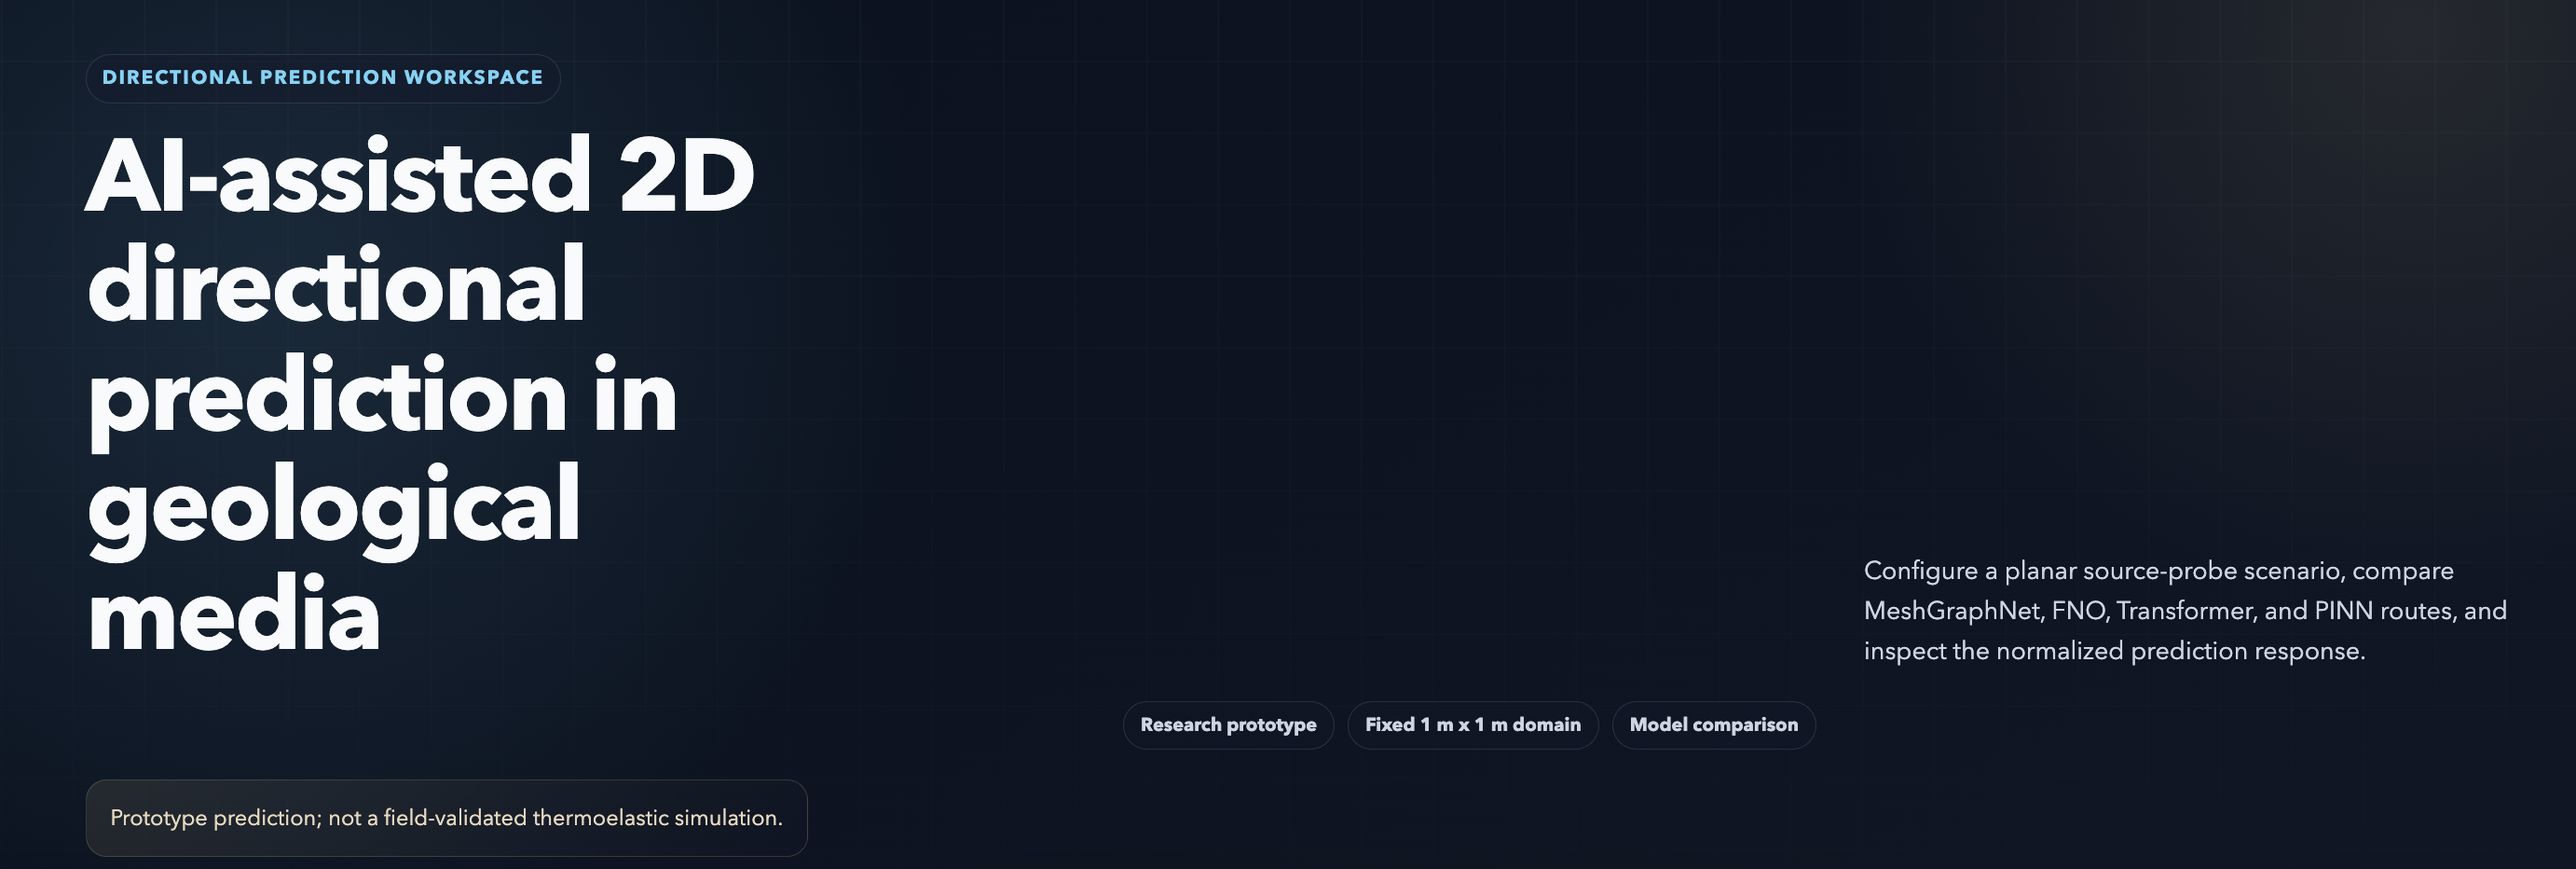
\includegraphics[width=0.96\textwidth]{chapters/web_implementation/figures/web_title}
\caption{Landing area: title, summary, and prototype-scope chips}
\label{fig:web-title}
\end{figure}

Below the landing area the workspace splits into a two-column grid. As
shown in Figure~\ref{fig:web-setup}, the left column hosts the
prediction-setup form, and the right column hosts the prediction-result
panel together with the planar domain visualisation. The split is
preserved on standard desktop widths and collapses to a single column
below the layout breakpoint so that the interface remains readable on
narrower windows.

\subsection{Prediction setup panel}

The prediction-setup panel implements the public side of the unified
prediction contract. Its structure follows the logical grouping of the
contract rather than an ad hoc visual order, so that the inputs
presented to the user map directly to the fields that the backend will
validate.

\begin{figure}[H]
\centering
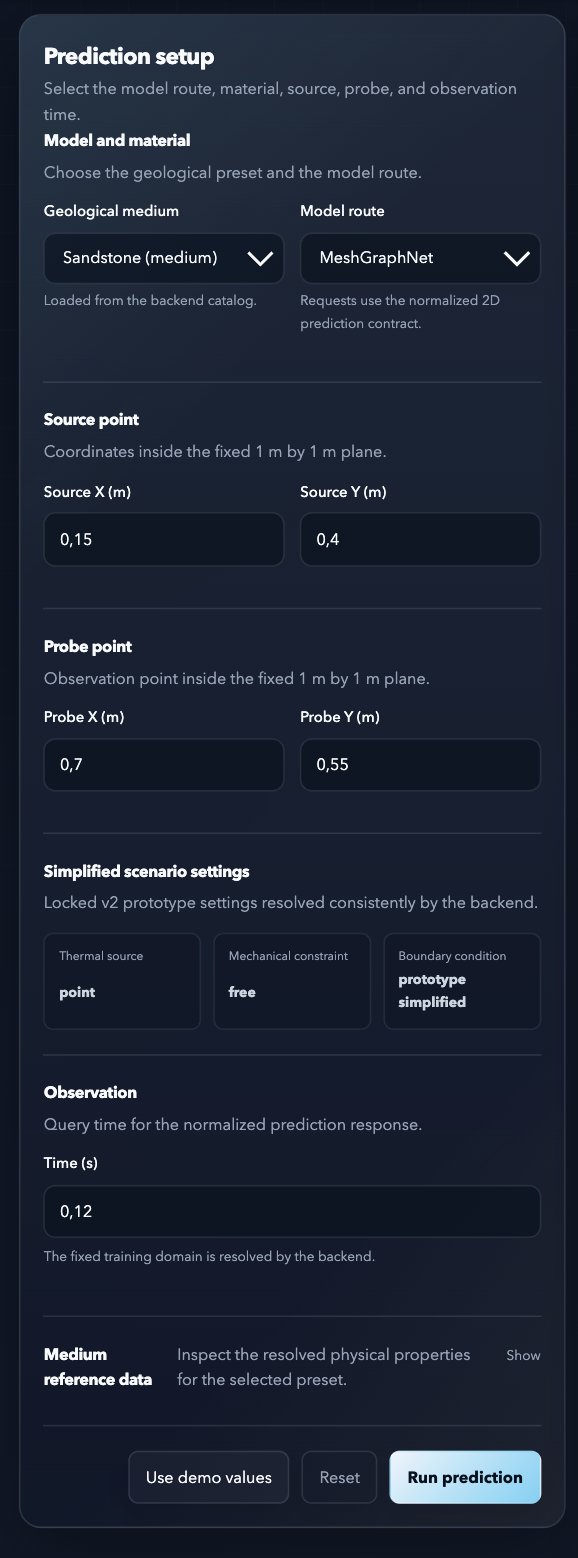
\includegraphics[height=0.74\textheight,keepaspectratio]{chapters/web_implementation/figures/web_setup}
\caption{Prediction setup panel: model, material, source, probe,
locked scenario, observation time}
\label{fig:web-setup}
\end{figure}

The first group is model and material selection. The material
drop-down exposes four medium presets carried by the catalog
(sandstone, limestone, basalt, granite); the model drop-down exposes
the four prediction routes (PINN, FNO, MeshGraphNet, Transformer). The
two selectors are independent, so that the same medium can be
evaluated through different routes and the same route can be evaluated
on different media. The source and probe coordinates are entered as
$(x,y)$ pairs inside the fixed unit square
$[0,1]\,\text{m}\times[0,1]\,\text{m}$ and are constrained at the
input level by minimum, maximum, and step attributes that prevent the
user from submitting points outside the trained operating envelope.

The \emph{Simplified scenario settings} block exposes three locked
prototype values that are pinned because the surrogate models were
trained under exactly these assumptions. Exposing them as a read-only
block is a deliberate design choice: it documents the operating
envelope without inviting requests that would push the inference
outside the training distribution.

\subsection{Two-dimensional domain visualisation}

The right column of the workspace opens with a single SVG canvas that
draws the source--probe geometry of the current request. The canvas
is re-rendered on every form change and on every successful response.
The planar domain visualisation is shown in Figure~\ref{fig:web-visualization}.

\begin{figure}[H]
\centering
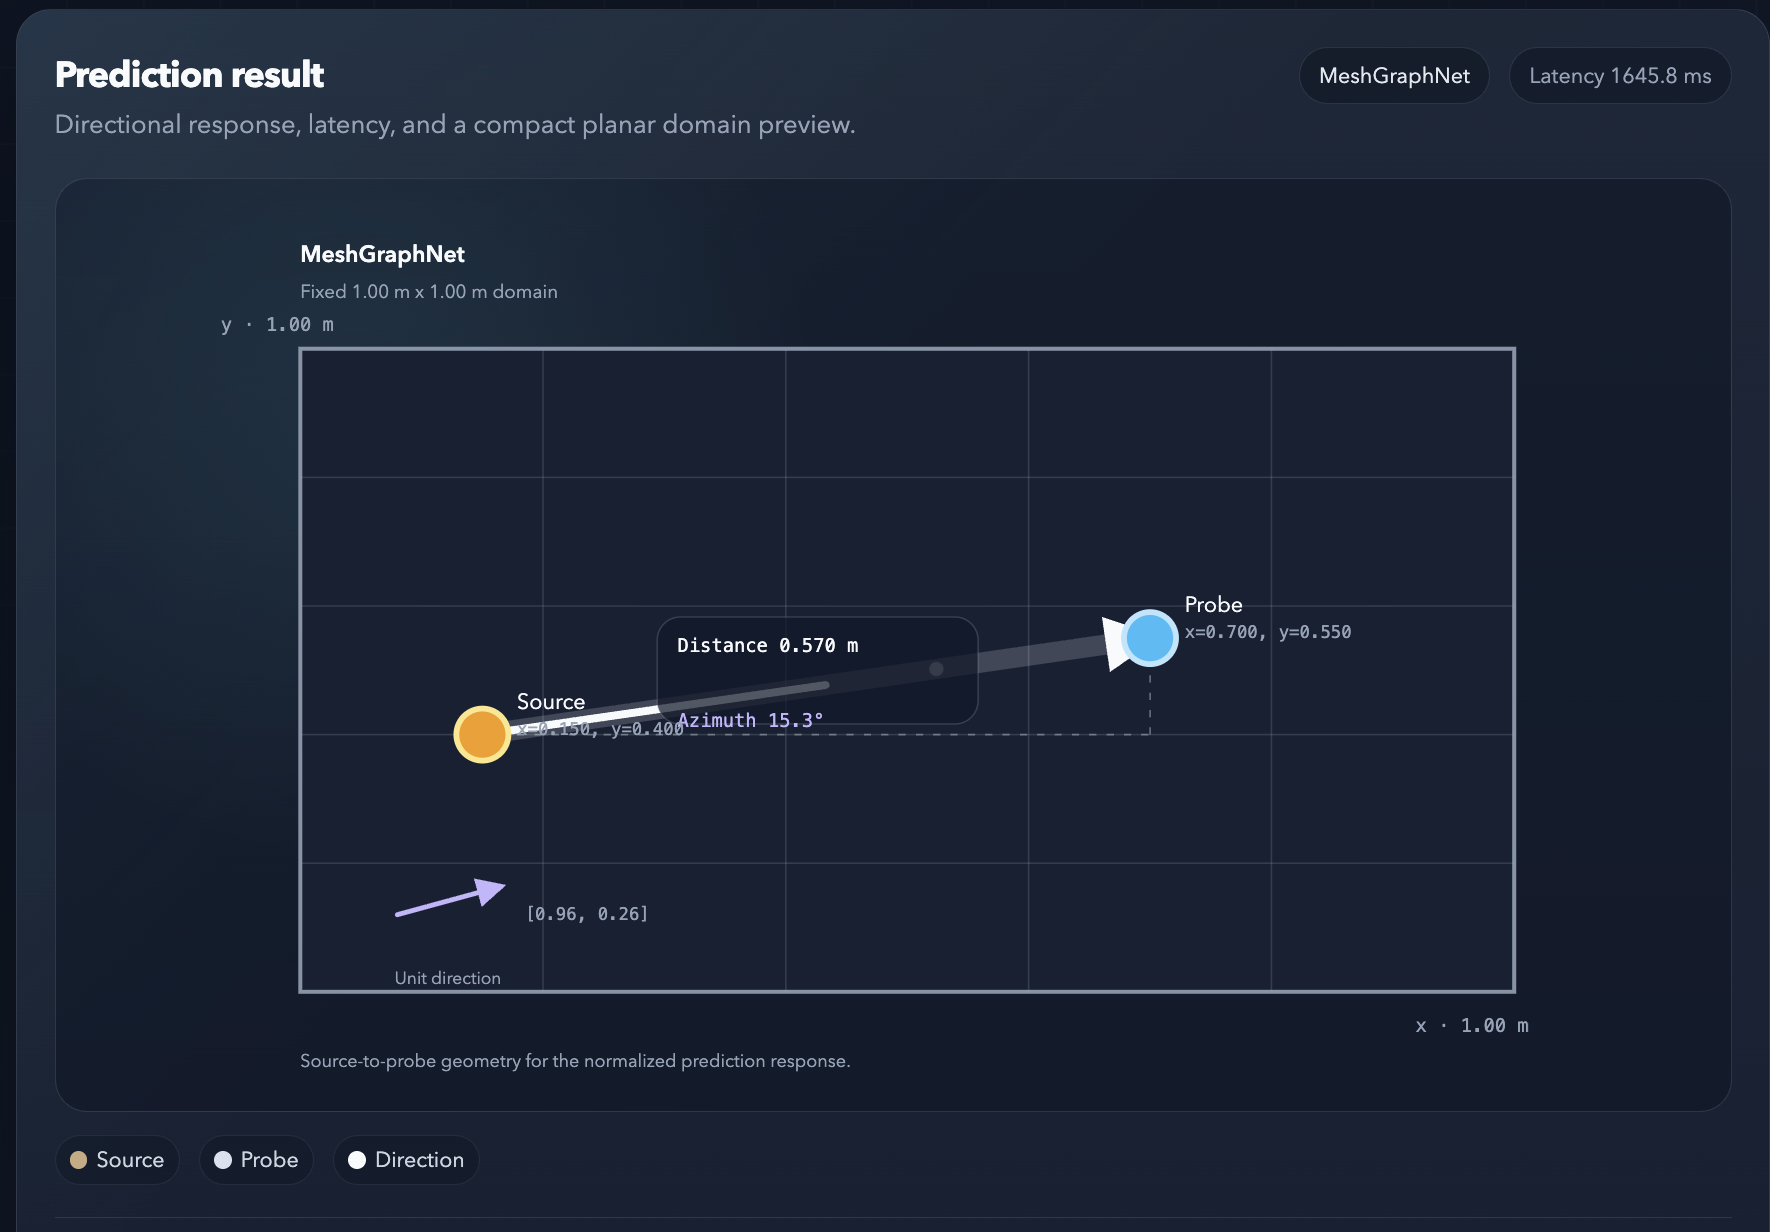
\includegraphics[width=0.92\textwidth]{chapters/web_implementation/figures/web_visualization}
\caption{Planar domain visualisation: source, probe, propagation
arrow with distance and azimuth, and unit-direction key}
\label{fig:web-visualization}
\end{figure}

The canvas uses separate top, bottom, left, and right margins so that
the header band, the unit square, and the bottom note do not share
vertical space. Source and probe labels are offset from the markers,
the distance and azimuth label is centred on the propagation arrow,
and the unit-direction key is anchored to the bottom-left corner of
the unit square. The geometry computation that produces the distance,
the azimuth, and the unit direction is the same one the backend uses
when it enriches the prediction response, so the visualisation and
the numeric panels always report identical directional quantities.

\subsection{Prediction result panel}

The prediction-result panel collects the normalised response of the
backend into thematic cards that inherit a common visual structure so
that the operator can read across routes without re-learning the
layout. The panel is shown in Figure~\ref{fig:web-result}.

\begin{figure}[H]
\centering
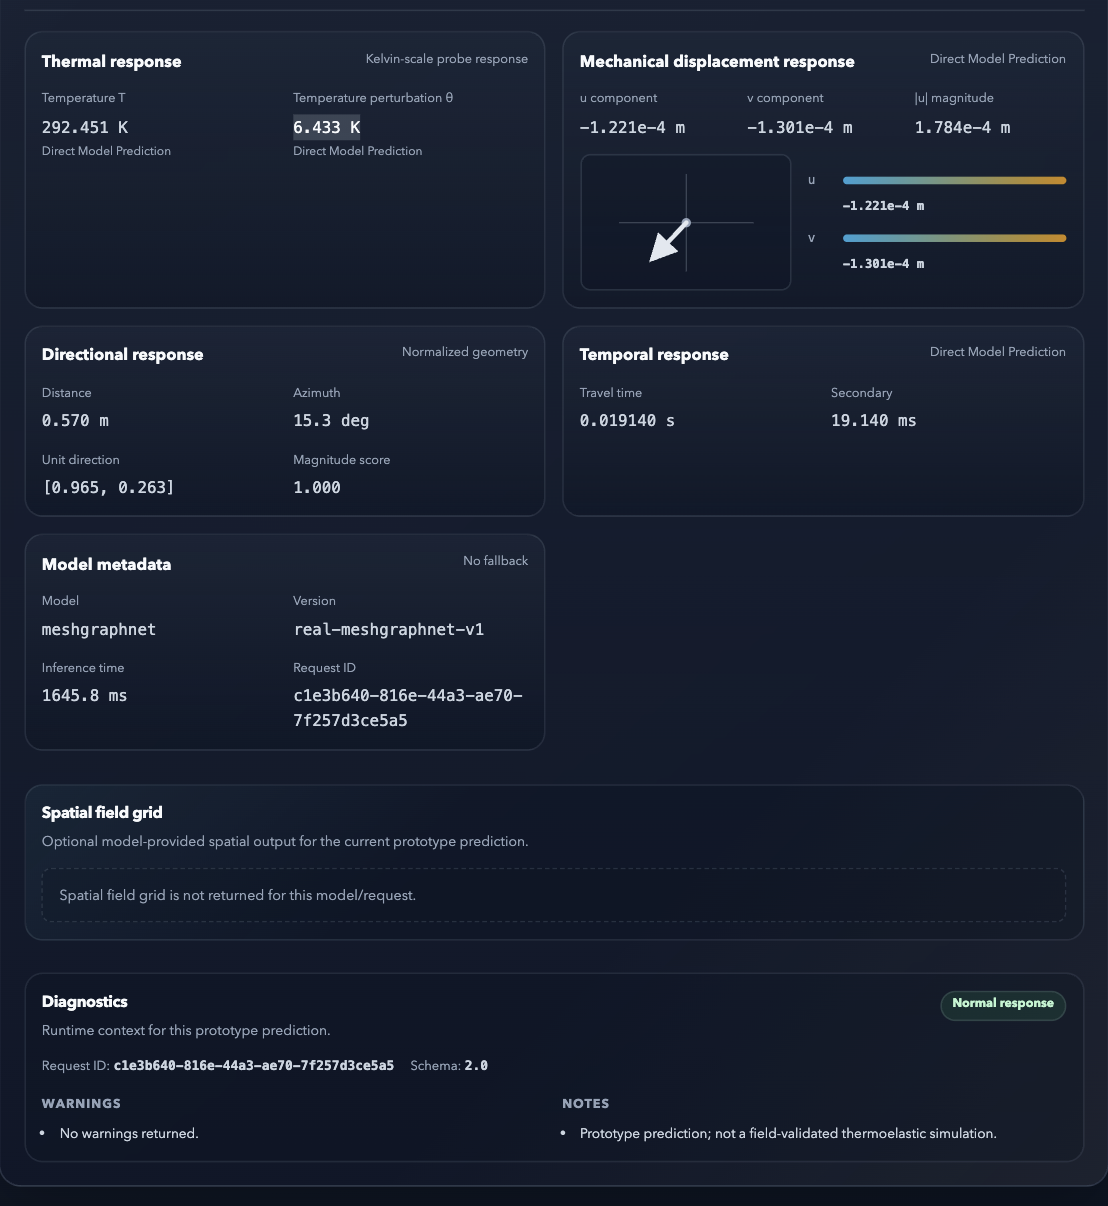
\includegraphics[width=0.94\textwidth]{chapters/web_implementation/figures/web_result}
\caption{Prediction result panel: thermal, displacement, directional,
temporal, and metadata cards with a diagnostics strip}
\label{fig:web-result}
\end{figure}

Long values such as the request identifier or scientific-notation
displacement components are allowed to wrap inside their cells, which
keeps the grid stable even when the formatted output is several
tokens long. The latency pill in the result-card header keeps the
practical cost of the prediction visible at all times and lets the
operator compare not only the directional quantities but also the
wall-clock behaviour of the four routes.

\subsection{Front-end and back-end interaction}

When the page loads, the application requests the medium catalog and
the model registry from the backend and populates the two drop-downs.
When the user clicks \emph{Run prediction}, the application serialises
the form into a v2 prediction-request payload, validates it locally
against the same field constraints that the backend enforces, and
submits it to the prediction endpoint. The response is normalised on
the backend side into the v2 prediction-response shape and the
front-end renders it directly without secondary post-processing.
Errors carry a machine-readable code, an HTTP status, and the request
identifier; they are displayed in a dedicated banner above the result
cards so that they cannot be confused with a successful prediction.

The front-end is intentionally thin: it does not perform any
thermoelastic computation, does not derive new physical quantities,
and does not implement any of the four model architectures. All
thermal, mechanical, directional, and temporal numbers visible in the
result panel are values produced by the backend or by the selected
model service. This separation guarantees that the four routes are
evaluated under identical pre-processing, identical post-processing,
and identical rendering, so that any observed difference between
routes is attributable to the model service rather than to the user
interface.

\subsection{Summary}

The web interface implements the user-facing surface of the prediction
prototype. Its design priorities are alignment with the unified
prediction contract, transparent presentation of the planar
source--probe geometry, and consistent rendering of the directional,
thermal, mechanical, and temporal components of the normalised
response. It is implemented as a static single-page application
without runtime dependencies and serves as the operational entry
point used to produce the scenarios reported in the comparative
evaluation.
